\chapter{Binary Liquid--Vapour Diagrams and Distillation}\label{ch:b2:liquid-vapour-diagrams}

A copper still turns a wine of a few per cent of alcohol into a spirit many
times stronger; a refinery column splits crude oil into its cuts, from gas to
heavy fuel. Both rely on one fact: the vapour over a boiling mixture is
richer in the more volatile component than the liquid. Repeat the
evaporation and condensation enough times and the separation becomes as
sharp as wanted --- with one exception: no distillation, however long the
column, takes ethanol beyond about 95 per cent by mass. This chapter draws
the diagrams that say how a mixture of two liquids boils, and uses them to
design a column and to see where it must stop.

\begin{recall}
\Cref{ch:b2:chemical-potential}: the \omterm{def:b2:chemical-potential:chemical-potential}{chemical potential}, \omterm{thm:b2:chemical-potential:raoult}{Raoult's law} and the
\omterm{def:b2:chemical-potential:ideal-mixture}{ideal mixture}, \omterm{def:b2:chemical-potential:activity-coefficient}{activity coefficients} and deviations from \omterm{thm:b2:chemical-potential:raoult}{Raoult's law}, the
Gibbs--Duhem relation. \Cref{ch:b2:equilibrium-shifts}: the \omterm{def:b2:equilibrium-shifts:variance}{variance}. The
Year 1 volume, on laboratory techniques: simple distillation, miscible and
immiscible liquids. The school volume: distillation and hydrodistillation.
\end{recall}

\begin{omfigure}
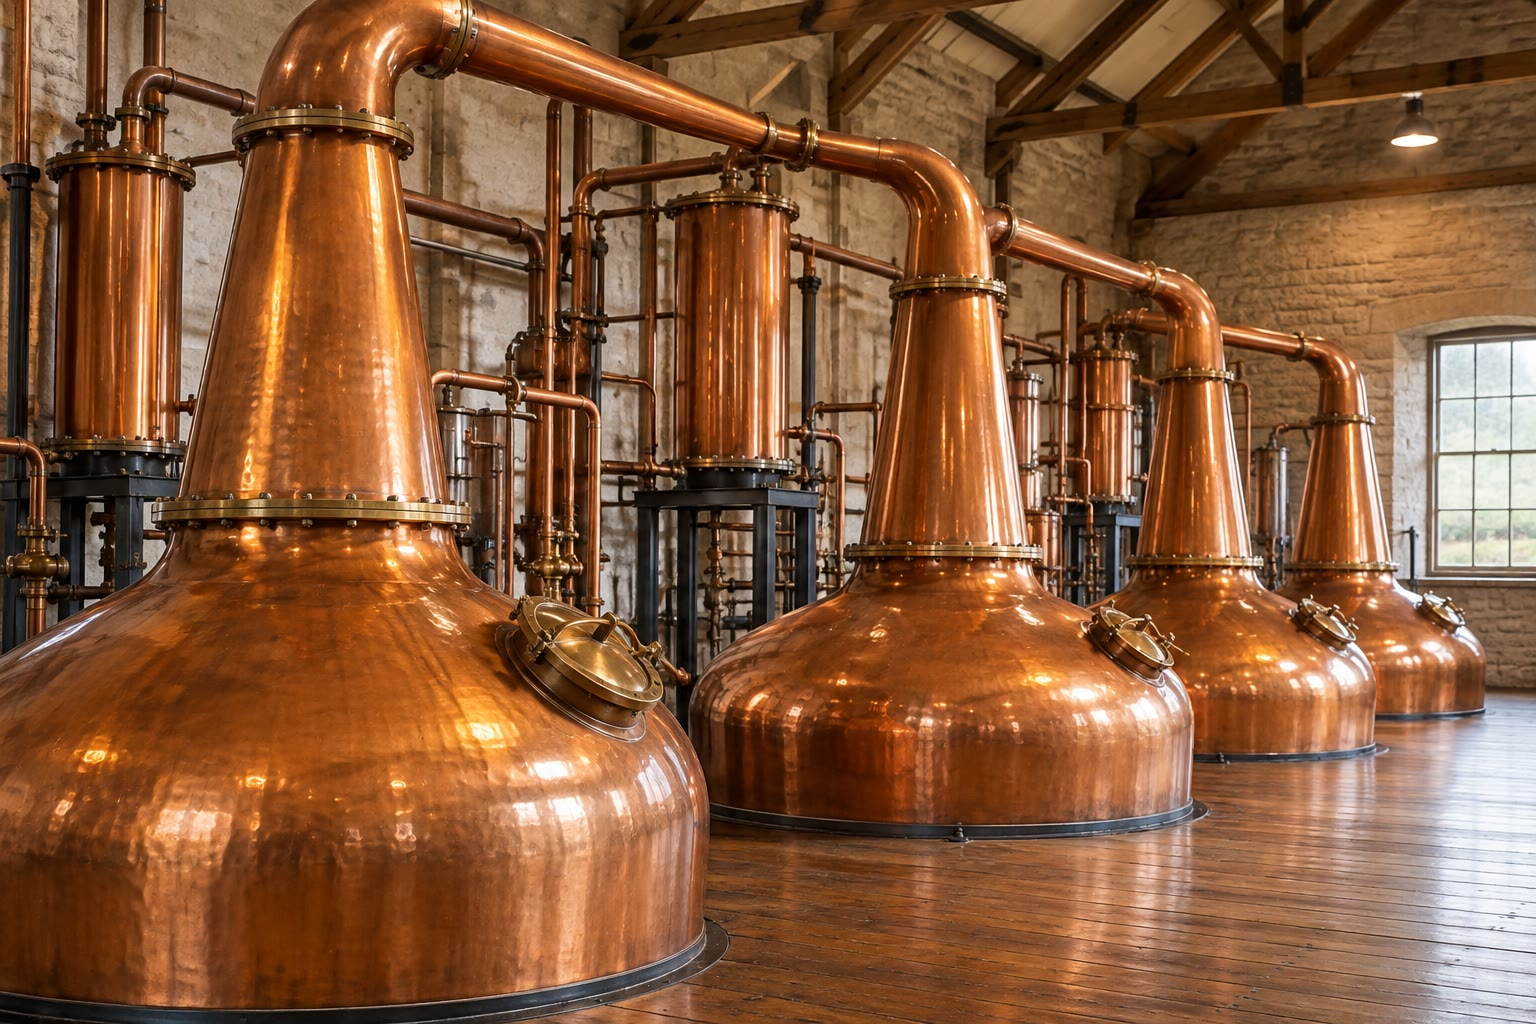
\includegraphics[width=0.62\linewidth]{images/book3/ai/b2-07-pot-stills.jpg}

{\small Copper pot stills in a distillery. Each charge of fermented wash is
boiled and its vapour condensed: the first distillate is several times richer
in ethanol than the wash, and a second distillation concentrates it further.}
\end{omfigure}

\section{Ideal mixtures}

In this chapter the two liquids are numbered 1 (the more volatile, of lower
boiling point) and 2; $x$ is the mole fraction of 1 in the liquid, $y$ its
mole fraction in the vapour, which is treated as an ideal gas.

\begin{definition}[Binary diagram]\label{def:b2:liquid-vapour-diagrams:binary-diagram}
A \emph{binary diagram}\index{binary diagram} shows, for a mixture of two
components, which phases are present and with which compositions, as a
function of the overall composition and of one other variable. An
\emph{isobaric diagram}\index{isobaric diagram} is drawn in the plane
(composition, temperature) at fixed pressure; an \emph{isothermal
diagram}\index{isothermal diagram} in the plane (composition, pressure) at
fixed temperature.
\end{definition}

\begin{definition}[Bubble and dew curves]\label{def:b2:liquid-vapour-diagrams:bubble-dew}
On a liquid--vapour diagram, the \emph{bubble curve}\index{bubble curve} gives
the composition of the liquid in equilibrium with vapour, the \emph{dew
curve}\index{dew curve} that of the vapour in equilibrium with liquid. For a
mixture of given composition at fixed pressure, the \emph{bubble
point}\index{bubble point} is the temperature at which the first bubble of
vapour appears on heating, the \emph{dew point}\index{dew point} the
temperature at which the first drop of liquid appears on cooling the vapour.
\end{definition}

\begin{proposition}[Ideal curves]\label{prop:b2:liquid-vapour-diagrams:ideal-curves}
For an \omterm{def:b2:chemical-potential:ideal-mixture}{ideal mixture} at temperature $T$, with $p_1^*$ and $p_2^*$ the vapour
pressures of the pure liquids, the \omterm{def:b2:liquid-vapour-diagrams:bubble-dew}{bubble curve} of the \omterm{def:b2:liquid-vapour-diagrams:binary-diagram}{isothermal diagram} is
the straight line $p = p_2^* + x(p_1^* - p_2^*)$, and the \omterm{def:b2:liquid-vapour-diagrams:bubble-dew}{dew curve} is the
hyperbola
\[
  p = \frac{1}{y/p_1^* + (1 - y)/p_2^*} .
\]
\end{proposition}

\begin{proof}
\omterm{thm:b2:chemical-potential:raoult}{Raoult's law} gives the partial pressures $p_1 = xp_1^*$ and $p_2 = (1 -
x)p_2^*$; their sum is the total pressure, linear in $x$. In the vapour,
$y = p_1/p$, so $x = yp/p_1^*$ and $1 - x = (1 - y)p/p_2^*$; adding,
$1 = p\,[y/p_1^* + (1 - y)/p_2^*]$.
\end{proof}

\begin{proposition}[The vapour is richer in the more volatile component]\label{prop:b2:liquid-vapour-diagrams:richer}
For an \omterm{def:b2:chemical-potential:ideal-mixture}{ideal mixture} with $p_1^* > p_2^*$ and $0 < x < 1$, $y > x$.
\end{proposition}

\begin{proof}
$y = xp_1^*/p$ with $p = xp_1^* + (1 - x)p_2^* < p_1^*$ since $p$ is a
weighted mean of $p_1^*$ and $p_2^*$, strictly between them. Hence $y >
x$.
\end{proof}

The \omterm{def:b2:liquid-vapour-diagrams:binary-diagram}{isobaric diagram} is the one that describes a distillation, which runs at
atmospheric pressure. It has no simple formula: for each temperature between
the two boiling points, $p_1^*(T)$ and $p_2^*(T)$ are computed (here with the
Antoine equation, $\log_{10}(p^*/\unit{bar}) = A - B/(T + C)$, fitted to
measured vapour pressures), and then the liquid and vapour compositions that
give a total pressure of \qty{1.013}{bar}:
\[
  x = \frac{p - p_2^*(T)}{p_1^*(T) - p_2^*(T)}, \qquad y = \frac{x\,p_1^*(T)}{p} .
\]
The \omterm{def:b2:liquid-vapour-diagrams:bubble-dew}{bubble curve} is no longer straight; the \omterm{def:b2:liquid-vapour-diagrams:bubble-dew}{dew curve} still lies above it,
the vapour still richer in the light component.

\begin{example}[Benzene and toluene at \qty{90}{\degreeCelsius}]\label{ex:b2:liquid-vapour-diagrams:benzene-toluene}
Benzene and toluene form a nearly \omterm{def:b2:chemical-potential:ideal-mixture}{ideal mixture}. At \qty{90}{\degreeCelsius}
the Antoine equations give $p_1^* = \qty{1.361}{bar}$ (benzene) and $p_2^* =
\qty{0.542}{bar}$ (toluene). At \qty{1.013}{bar}: $x = (1.013 - 0.542)/(1.361 -
0.542) = 0.575$ and $y = 0.575 \times 1.361/1.013 = 0.773$. A liquid of 57.5~\%
benzene (in moles) boils at \qty{90}{\degreeCelsius} and gives a vapour of
77~\%.
% ledger: antoine:benzene.A, antoine:benzene.B, antoine:benzene.C, antoine:toluene.A, antoine:toluene.B, antoine:toluene.C
\end{example}

\begin{omfigure}
\begin{tikzpicture}
\begin{axis}[omphase, width=0.47\linewidth, height=6cm, ymin=78, ymax=113,
  xlabel={$x$, $y$ (benzene)}, ylabel={$T$ (\unit{\degreeCelsius})},
  title={\small isobaric, \qty{1.013}{bar}}]
\addplot[omliquidus] table[x=x, y=T] {figdata/out/bachelor-2-liquid-vapour-a.dat};
\addplot[omsolidus] table[x=y, y=T] {figdata/out/bachelor-2-liquid-vapour-a.dat};
\draw[tieline] (axis cs:0.405,95) -- (axis cs:0.626,95);
\fill (axis cs:0.5,95) circle (1.3pt);
\draw[->, thick] (axis cs:0.5,82) -- (axis cs:0.5,104) node[above, font=\scriptsize] {heating};
\node[font=\scriptsize] at (axis cs:0.2,85) {liquid};
\node[font=\scriptsize] at (axis cs:0.85,108) {vapour};
\node[font=\scriptsize, omDef, anchor=north] at (axis cs:0.22,96) {bubble};
\node[font=\scriptsize, omThm, anchor=south west] at (axis cs:0.62,101) {dew};
\end{axis}
\end{tikzpicture}\hfill
\begin{tikzpicture}
\begin{axis}[omphase, width=0.47\linewidth, height=6cm, ymin=0.3, ymax=1.1,
  xlabel={$x$, $y$ (benzene)}, ylabel={$p$ (\unit{bar})},
  title={\small isothermal, \qty{80}{\degreeCelsius}}]
\addplot[omliquidus] table[x=x, y=pbub] {figdata/out/bachelor-2-liquid-vapour-b.dat};
\addplot[omsolidus] table[x=x, y=pdew] {figdata/out/bachelor-2-liquid-vapour-b.dat};
\node[font=\scriptsize] at (axis cs:0.75,0.98) {liquid};
\node[font=\scriptsize] at (axis cs:0.2,0.36) {vapour};
\end{axis}
\end{tikzpicture}

{\small Benzene--toluene, computed from \omterm{thm:b2:chemical-potential:raoult}{Raoult's law} and the Antoine
equations. Left, at atmospheric pressure: \omterm{def:b2:liquid-vapour-diagrams:bubble-dew}{bubble curve} (blue) and \omterm{def:b2:liquid-vapour-diagrams:bubble-dew}{dew curve}
(red); the liquid of composition 0.5 starts to boil at
\qty{92.1}{\degreeCelsius} and is all vapour at \qty{98.8}{\degreeCelsius}; at
\qty{95}{\degreeCelsius} (dashed tie line) it is split into a liquid of 0.405
and a vapour of 0.626. Right, at \qty{80}{\degreeCelsius}: the \omterm{def:b2:liquid-vapour-diagrams:bubble-dew}{bubble curve} is
straight, the \omterm{def:b2:liquid-vapour-diagrams:bubble-dew}{dew curve} a hyperbola, the liquid now on top.}
% ledger: antoine:benzene.A, antoine:toluene.A (all six parameters in figdata/bachelor-2/liquid-vapour.py)
\end{omfigure}

\section{Reading a diagram}

\begin{proposition}[Variance of a two-phase binary]\label{prop:b2:liquid-vapour-diagrams:variance}
A mixture of two components in two phases has \omterm{def:b2:equilibrium-shifts:variance}{variance} 2. At fixed pressure
the temperature alone fixes the compositions of both phases: they are read
at the ends of the horizontal segment through the representative point,
called a tie line.
\end{proposition}

\begin{proof}
Intensive variables: $T$, $p$, $x$, $y$. Relations: equality of the \omterm{def:b2:chemical-potential:chemical-potential}{chemical
potentials} of 1 and of 2 between the phases. $v = 4 - 2 = 2$ (the phase rule
$v = n - r + 2 - \varphi$ gives the same with $n = 2$, $r = 0$, $\varphi = 2$).
Fixing $p$ leaves one degree of freedom: $x(T)$ and $y(T)$ are the two curves.
\end{proof}

\begin{theorem}[Lever rule]\label{thm:b2:liquid-vapour-diagrams:lever}
A mixture of overall composition $z$, split into a liquid of composition $x$
and a vapour of composition $y$, contains amounts $n_L$ of liquid and $n_V$ of
vapour such that
\[
  n_L\,(z - x) = n_V\,(y - z), \qquad \frac{n_V}{n_L + n_V} = \frac{z - x}{y - x} .
\]
This is the \emph{lever rule}\index{lever rule}: each phase is the more
abundant the closer its composition is to the overall one, like the weights on
a lever pivoting at $z$.
\end{theorem}

\begin{proof}
Conservation of component 1: $(n_L + n_V)z = n_Lx + n_Vy$, so $n_L(z - x) =
n_V(y - z)$; divide by $n_L + n_V$ and rearrange.
\end{proof}

The \omterm{thm:b2:liquid-vapour-diagrams:lever}{lever rule} holds with mole fractions and amounts, as here, or with mass
fractions and masses: the conservation used is the same.

\begin{method}[Reading a binary diagram]\label{met:b2:liquid-vapour-diagrams:read-diagram}
\begin{enumerate}
  \item Place the point (overall composition, temperature) and name its
        domain: liquid, vapour, or liquid + vapour.
  \item In a two-phase domain, draw the tie line through the point; its ends
        give the compositions of the liquid (on the \omterm{def:b2:liquid-vapour-diagrams:bubble-dew}{bubble curve}) and of the
        vapour (on the \omterm{def:b2:liquid-vapour-diagrams:bubble-dew}{dew curve}).
  \item Get the proportions of the phases from the \omterm{thm:b2:liquid-vapour-diagrams:lever}{lever rule}.
  \item To follow a heating, move the point upwards: the first bubble appears
        on the \omterm{def:b2:liquid-vapour-diagrams:bubble-dew}{bubble curve}, the last drop disappears on the \omterm{def:b2:liquid-vapour-diagrams:bubble-dew}{dew curve};
        between them the liquid grows poorer in the light component.
\end{enumerate}
\end{method}

\begin{example}[A flash at \qty{95}{\degreeCelsius}]\label{ex:b2:liquid-vapour-diagrams:flash}
\qty{100}{mol} of an equimolar benzene--toluene mixture are brought to
\qty{95}{\degreeCelsius} at atmospheric pressure. The tie line gives $x =
0.405$, $y = 0.626$; the vapour fraction is $(0.500 - 0.405)/(0.626 - 0.405) =
0.43$: \qty{43}{mol} of vapour holding $43 \times 0.626 = \qty{27}{mol}$ of
benzene, \qty{57}{mol} of liquid holding \qty{23}{mol}. One equilibrium stage
enriches, but only a little.
\end{example}

\section{Real mixtures and azeotropes}

When the \omterm{def:b2:chemical-potential:activity-coefficient}{activity coefficients} differ from 1 (\cref{ch:b2:chemical-potential}),
the partial pressures depart from Raoult's straight lines. With a positive
deviation ($\gamma > 1$: unlike molecules attract each other less than like
ones) the total pressure lies above the ideal line; with a negative deviation
below. If the deviation is strong enough, the total pressure goes through an
extremum.

\begin{definition}[Azeotrope]\label{def:b2:liquid-vapour-diagrams:azeotrope}
An \emph{azeotrope}\index{azeotrope} is a liquid mixture that boils without
changing composition: the vapour it gives has its own composition. A
\emph{positive azeotrope}\index{positive azeotrope} (positive deviation) has
a maximum of pressure on the \omterm{def:b2:liquid-vapour-diagrams:binary-diagram}{isothermal diagram} and a minimum of boiling
temperature on the isobaric one; a \emph{negative azeotrope}\index{negative azeotrope}
the reverse.
\end{definition}

\begin{theorem}[Gibbs--Konovalov]\label{thm:b2:liquid-vapour-diagrams:konovalov}
On a binary liquid--vapour diagram, at an extremum of the total pressure (at
fixed temperature) or of the boiling temperature (at fixed pressure), the
liquid and the vapour have the same composition. Conversely, where the
two compositions are equal, the curves have a common horizontal tangent.
\end{theorem}

\begin{proof}[Proof at fixed temperature]
The Gibbs--Duhem relation for the liquid at fixed $T$ (the small effect of $p$
on the liquid neglected) is $x\,d\mu_1 + (1 - x)\,d\mu_2 = 0$. At equilibrium
$\mu_i = \mu_i^\circ + RT\ln(p_i/p^\circ)$ with $p_1 = yp$, $p_2 = (1 - y)p$, so
\[
  x\,d\ln(yp) + (1 - x)\,d\ln((1 - y)p) = 0
  \quad\Longrightarrow\quad
  d\ln p = -\Big(\frac{x}{y} - \frac{1 - x}{1 - y}\Big)dy
  = \frac{y - x}{y(1 - y)}\,dy .
\]
As $y$ increases with $x$ (otherwise the liquid would be unstable),
$dp/dx = 0$ exactly where $y = x$. The isobaric case follows from a similar
calculation that keeps the temperature dependence of the $\mu_i^\circ$; it is
not carried out here.
\end{proof}

The formula says more: where $y > x$, the pressure increases with $x$ ---
adding the component that is enriched in the vapour makes the liquid more
volatile, which is Konovalov's first law.

\begin{example}[Ethanol and water]\label{ex:b2:liquid-vapour-diagrams:ethanol-water}
Ethanol and water deviate positively from \omterm{thm:b2:chemical-potential:raoult}{Raoult's law} and form an \omterm{def:b2:liquid-vapour-diagrams:azeotrope}{azeotrope}
of 95~\% ethanol by mass at atmospheric pressure. With $M = 46.07$ and
\qty{18.02}{g/mol}, its mole fraction of ethanol is
\[
  x_{\text{az}} = \frac{95/46.07}{95/46.07 + 5/18.02} = 0.881 .
\]
It boils a little below pure ethanol (\qty{78.3}{\degreeCelsius}). The diagram
below is computed from a one-parameter activity model, $\ln\gamma_1 = A(1 -
x)^2$, $\ln\gamma_2 = Ax^2$, whose parameter ($A = 1.09$) is fitted so that the
\omterm{def:b2:liquid-vapour-diagrams:azeotrope}{azeotrope} falls at that composition: the model reproduces the shape, and
places the \omterm{def:b2:liquid-vapour-diagrams:azeotrope}{azeotrope} at \qty{77.9}{\degreeCelsius}.
% ledger: azeo:ethanol-water.w, aw:C, aw:H, aw:O, antoine:ethanol.A, antoine:ethanol.B, antoine:ethanol.C, antoine:water.A, antoine:water.B, antoine:water.C
\end{example}

\begin{omfigure}
\begin{tikzpicture}
\begin{axis}[omphase, width=0.47\linewidth, height=6cm, ymin=76, ymax=101,
  xlabel={$x$, $y$ (ethanol)}, ylabel={$T$ (\unit{\degreeCelsius})},
  title={\small ethanol--water (model)}]
\addplot[omliquidus] table[x=x, y=T] {figdata/out/bachelor-2-liquid-vapour-c.dat};
\addplot[omsolidus] table[x=y, y=T] {figdata/out/bachelor-2-liquid-vapour-c.dat};
\fill (axis cs:0.881,77.92) circle (1.5pt);
\draw[densely dotted] (axis cs:0.881,77.92) -- (axis cs:0.881,76);
\node[font=\scriptsize, anchor=south] at (axis cs:0.80,80.5) {azeotrope};
\draw[thin] (axis cs:0.80,80.5) -- (axis cs:0.875,78.2);
\node[font=\scriptsize] at (axis cs:0.25,79.5) {liquid};
\node[font=\scriptsize] at (axis cs:0.5,95) {vapour};
\end{axis}
\end{tikzpicture}\hfill
\begin{tikzpicture}
\begin{axis}[omphase, width=0.47\linewidth, height=6cm, ymin=78, ymax=120,
  xlabel={$x$, $y$ (component 1)}, ylabel={$T$ (\unit{\degreeCelsius})},
  title={\small negative deviation (model)}]
\addplot[omliquidus] table[x=x, y=T] {figdata/out/bachelor-2-liquid-vapour-d.dat};
\addplot[omsolidus] table[x=y, y=T] {figdata/out/bachelor-2-liquid-vapour-d.dat};
\fill (axis cs:0.29,116.7) circle (1.5pt);
\node[font=\scriptsize, anchor=west] at (axis cs:0.33,118) {azeotrope};
\node[font=\scriptsize] at (axis cs:0.6,85) {liquid};
\node[font=\scriptsize] at (axis cs:0.75,116) {vapour};
\end{axis}
\end{tikzpicture}

{\small Left: ethanol--water at atmospheric pressure, from a one-parameter
model fitted to the \omterm{def:b2:liquid-vapour-diagrams:azeotrope}{azeotrope} composition (0.881); the \omterm{def:b2:liquid-vapour-diagrams:azeotrope}{azeotrope} boils below
both pure liquids. Right: a model pair with a strong negative deviation
($A = -2.0$, vapour pressures of benzene and toluene); the \omterm{def:b2:liquid-vapour-diagrams:azeotrope}{azeotrope} boils
above both.}
% ledger: azeo:ethanol-water.w, antoine:ethanol.A, antoine:water.A (model in figdata/bachelor-2/liquid-vapour.py)
\end{omfigure}

\section{Fractional distillation}

\begin{definition}[Fractional distillation]\label{def:b2:liquid-vapour-diagrams:fractional-distillation}
\emph{Fractional distillation}\index{fractional distillation} separates the
components of a liquid mixture in a column where a rising vapour and a
descending liquid are brought into repeated contact. A \emph{theoretical
plate}\index{theoretical plate} is a stage of the column whose leaving vapour
and liquid are in equilibrium with each other. The \emph{reflux
ratio}\index{reflux ratio} is the ratio of the amount of condensate returned
to the top of the column to the amount drawn off as distillate.
\end{definition}

On each plate the vapour from below bubbles through the liquid from above; it
leaves richer in the light component, the liquid poorer. At the top the vapour
is condensed, part of it returned as reflux, the rest drawn off as the
distillate; at the bottom a reboiler boils part of the liquid. At
\textit{total reflux} nothing is drawn off: the column then works at its best,
and the vapour leaving a plate has the composition of the liquid coming down
on it.


For an ideal pair, the \textit{relative volatility} $\alpha = p_1^*/p_2^*$
changes little over the column: from 2.60 at the boiling point of benzene to
2.35 at that of toluene. On each \omterm{def:b2:liquid-vapour-diagrams:fractional-distillation}{theoretical plate}
\[
  \frac{y}{1 - y} = \frac{xp_1^*}{(1 - x)p_2^*} = \alpha\,\frac{x}{1 - x} .
\]

\begin{omfigure}
\begin{minipage}[b]{0.58\linewidth}\centering
\begin{tikzpicture}[font=\small, >={Stealth}, scale=0.8, every node/.style={transform shape}]
  \draw[thick, fill=gray!8] (0,0) rectangle (1.8,7);
  \foreach \k in {1,...,6} {
    \pgfmathsetmacro{\yy}{\k}
    \ifodd\k
      \draw[thick] (0,\yy) -- (1.45,\yy); \draw[thick] (1.45,\yy) -- (1.45,\yy-0.55);
    \else
      \draw[thick] (0.35,\yy) -- (1.8,\yy); \draw[thick] (0.35,\yy) -- (0.35,\yy-0.55);
    \fi
    \fill[omDef!25] (0.02,\yy) rectangle (1.78,\yy+0.12);
  }
  \foreach \k in {1,...,6} \node[font=\scriptsize, anchor=east] at (-0.1,\k) {plate \k};
  \draw[->, thick, omThm] (0.9,7.0) -- (0.9,7.9) -- (2.8,7.9);
  \draw[thick, fill=white] (2.8,7.6) rectangle (3.6,8.2);
  \node[anchor=west, font=\scriptsize] at (3.65,7.9) {condenser};
  \draw[->, thick, omDef] (3.2,7.6) -- (3.2,5.6);
  \draw[thick, fill=omDef!20] (2.7,5.0) rectangle (3.7,5.6);
  \node[font=\scriptsize, anchor=west] at (3.75,5.3) {reflux drum};
  \draw[->, thick, omDef] (2.7,5.3) -- (2.1,5.3) -- (2.1,6.6) -- (1.8,6.6);
  \node[font=\scriptsize, anchor=west, omDef] at (2.15,6.1) {reflux};
  \draw[->, thick, omDef] (3.2,5.0) -- (3.2,4.4) -- (4.4,4.4) node[right] {distillate};
  \draw[->, thick] (-2.2,3.5) -- (0,3.5) node[pos=0, left] {feed};
  \draw[thick, fill=omDef!20] (0.2,-1.3) rectangle (1.6,-0.6);
  \node[font=\scriptsize] at (0.9,-0.95) {reboiler};
  \draw[thick, omDef] (0.9,0) -- (0.9,-0.6);
  \draw[->, thick, omThm] (1.6,-0.8) -- (2.1,-0.8) -- (2.1,0.4) -- (1.8,0.4);
  \draw[->, thick, omDef] (0.9,-1.3) -- (0.9,-1.8) -- (2.6,-1.8) node[right] {bottoms};
  \draw[->, omThm, thick] (2.6,1.5) -- (2.6,3.0) node[midway, right, font=\scriptsize, align=left] {vapour\\ rises};
  \draw[->, omDef, thick] (-1.4,5.8) -- (-1.4,4.3) node[midway, left, font=\scriptsize, align=right] {liquid\\ falls};
\end{tikzpicture}
\end{minipage}\hfill
\begin{minipage}[b]{0.34\linewidth}\centering
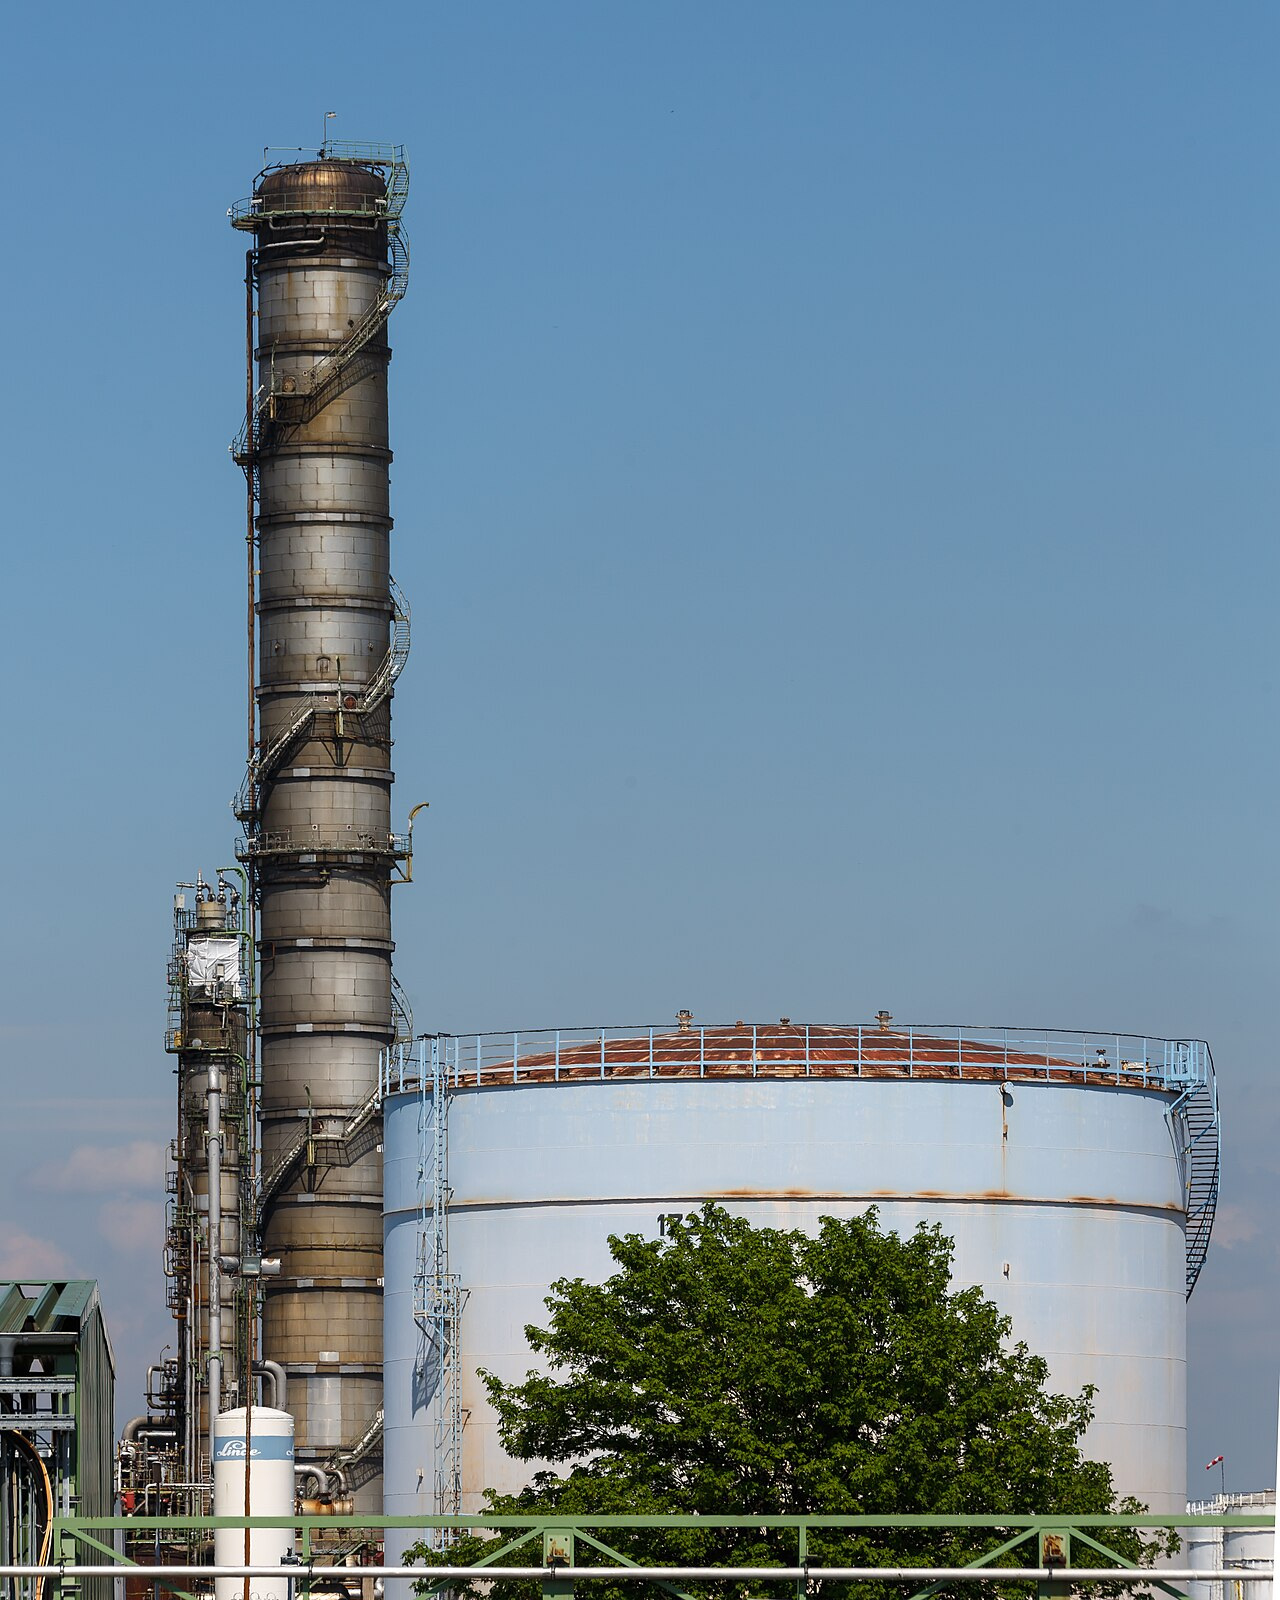
\includegraphics[width=\linewidth]{images/book3/refinery-column.jpg}
\end{minipage}

{\small Left: a plate column. Liquid flows across each plate and down the
downcomer to the plate below; vapour rises through the plates and bubbles
through the liquid. The condensed vapour is partly returned as reflux; the
reboiler at the bottom provides the vapour. Right: a distillation column of a
refinery (Cologne, 2014), which holds dozens of plates. (Photograph: CEphoto,
Uwe Aranas, CC BY-SA 3.0, Wikimedia Commons.)}
\end{omfigure}

\begin{proposition}[Fenske]\label{prop:b2:liquid-vapour-diagrams:fenske}
At total reflux, with a constant relative volatility $\alpha$, the number of
\omterm{def:b2:liquid-vapour-diagrams:fractional-distillation}{theoretical plates} needed to go from a bottom liquid $x_B$ to a distillate
$x_D$ is at least
\[
  N_{\min} = \frac{1}{\ln\alpha}\,\ln\!\left[\frac{x_D}{1 - x_D}\cdot\frac{1 - x_B}{x_B}\right] .
\]
\end{proposition}

\begin{proof}
Number the plates from the bottom, the reboiler being plate 1. At total reflux
the liquid coming down on plate $k + 1$ has the composition of the vapour
leaving plate $k$: $x_{k+1} = y_k$. With $r = x/(1 - x)$, each plate gives
$r(y_k) = \alpha\,r(x_k)$, so $r(x_{k+1}) = \alpha\,r(x_k)$, and after $N$
plates the condensed vapour has $r(x_D) = \alpha^N r(x_B)$. Taking logarithms
gives $N$. With a finite reflux, the liquid flowing down is leaner than the
vapour rising, each plate enriches less, and more plates are needed.
\end{proof}

On the $(x, y)$ diagram the same construction is a staircase between the
equilibrium curve and the diagonal $y = x$: each step is one \omterm{def:b2:liquid-vapour-diagrams:fractional-distillation}{theoretical
plate}.

\begin{omfigure}
\begin{tikzpicture}
\begin{axis}[width=0.55\linewidth, height=0.55\linewidth, xmin=0, xmax=1,
  ymin=0, ymax=1, axis x line=bottom, axis y line=left,
  xlabel={$x$ (benzene, liquid)}, ylabel={$y$ (benzene, vapour)},
  tick label style={font=\small}, label style={font=\small}]
\addplot[omThm, thick] table[x=x, y=y] {figdata/out/bachelor-2-liquid-vapour-f-eq.dat};
\addplot[black!50] coordinates {(0,0) (1,1)};
\addplot[omDef, thick] table[x=x, y=y] {figdata/out/bachelor-2-liquid-vapour-f.dat};
\draw[densely dotted] (axis cs:0.95,0) -- (axis cs:0.95,0.95);
\draw[densely dotted] (axis cs:0.05,0) -- (axis cs:0.05,0.05);
\node[font=\scriptsize, anchor=south east] at (axis cs:0.945,0.02) {$x_D$};
\node[font=\scriptsize, anchor=south west] at (axis cs:0.05,0.02) {$x_B$};
\end{axis}
\end{tikzpicture}

{\small Plates at total reflux for benzene--toluene, from a distillate of
0.95 down: each horizontal step goes from a vapour to the liquid in
equilibrium with it (one plate), each vertical step from that liquid to the
vapour of the plate below. Seven steps take the liquid below $x_B = 0.05$;
Fenske's formula gives 6.5.}
% ledger: antoine:benzene.A, antoine:toluene.A (computed in figdata/bachelor-2/liquid-vapour.py)
\end{omfigure}

\begin{proposition}[A column cannot cross an azeotrope]\label{prop:b2:liquid-vapour-diagrams:azeotrope-limit}
In a mixture with an \omterm{def:b2:liquid-vapour-diagrams:azeotrope}{azeotrope}, a column fed on one side of the azeotropic
composition delivers at best the \omterm{def:b2:liquid-vapour-diagrams:azeotrope}{azeotrope} at one end and the pure component
of that side at the other.
\end{proposition}

\begin{proof}
At the \omterm{def:b2:liquid-vapour-diagrams:azeotrope}{azeotrope} the equilibrium curve meets the diagonal: $y = x$. Near it
each step of the staircase becomes vanishingly small, so no finite number of
plates reaches it, and none crosses it.
\end{proof}

\begin{method}[Predicting a fractional distillation]\label{met:b2:liquid-vapour-diagrams:predict-distillation}
\begin{enumerate}
  \item Find the lowest-boiling point accessible from the feed on the
        \omterm{def:b2:liquid-vapour-diagrams:binary-diagram}{isobaric diagram}: a pure component or a \omterm{def:b2:liquid-vapour-diagrams:azeotrope}{positive azeotrope}. It comes
        out at the top.
  \item The highest-boiling point on the same side (pure component or
        \omterm{def:b2:liquid-vapour-diagrams:azeotrope}{negative azeotrope}) remains in the boiler.
  \item With an \omterm{def:b2:liquid-vapour-diagrams:azeotrope}{azeotrope}, look on which side of it the feed lies: only that
        side's pure component can be obtained.
  \item For the number of plates, use Fenske's formula or the staircase,
        then add plates for the finite reflux actually used.
\end{enumerate}
\end{method}

For ethanol and water fed at less than 0.881, the top delivers at best the
\omterm{def:b2:liquid-vapour-diagrams:azeotrope}{azeotrope} and the bottom water: no column gives absolute ethanol. Drying the
last per cent needs another method --- a molecular sieve that adsorbs water, or
a third component added to break the \omterm{def:b2:liquid-vapour-diagrams:azeotrope}{azeotrope}.

\begin{omfigure}
\begin{tikzpicture}[font=\small, scale=0.95, >={Stealth}]
  \pic[transform shape] at (0,0) {heatingmantle};
  \pic[transform shape] at (0,0) {rbflask={0.45}{orange!25}};
  \foreach \x/\y in {-0.35/0.25,0.05/0.18,0.35/0.3}
    \fill[black!55] (\x,\y) circle (0.06);
  % Vigreux column from the flask neck (0,3) to (0,6)
  \draw[om glass] (-0.22,3.0) -- (-0.22,6.0) (0.22,3.0) -- (0.22,6.0);
  \foreach \yy in {3.4,3.9,4.4,4.9,5.4} {
    \draw[om glass] (-0.22,\yy) -- (-0.06,\yy+0.18) -- (-0.22,\yy+0.3);
    \draw[om glass] (0.22,\yy+0.15) -- (0.06,\yy+0.33) -- (0.22,\yy+0.45);
  }
  \pic[transform shape] (s) at (0,6.0) {stillhead};
  \pic[transform shape] at ($(s-top)+(0,-0.75)$) {thermometer};
  \pic[transform shape, rotate=-20] (c) at (s-arm) {liebig={3.4}};
  % ground-glass joint between the head's side arm and the condenser
  \draw[om glass, fill=white, rotate around={-20:(s-arm)}] ($(s-arm)+(-0.12,-0.17)$) rectangle ($(s-arm)+(0.14,0.17)$);
  \coordinate (cend) at ($(s-arm)+(-20:3.4)$);
  \pic[transform shape] (a) at (cend) {adapter};
  \pic[transform shape] at ($(a-tip)+(0,-2.4)$) {erlenmeyer={0.22}{orange!12}};
  \draw[<-, omProp, thick] (-0.25,4.6) -- (-1.6,4.6) node[left, text=black,
    align=right] {Vigreux column\\ (indentations multiply\\ the contacts)};
  \draw[<-, omProp, thick] (0.12,6.72) -- (-1.4,7.4) node[left, text=black,
    align=right] {thermometer bulb\\ level with the side arm};
  \draw[<-, omProp, thick] (1.08,0.3) -- (2.3,-0.2) node[right, text=black]
    {heating mantle};
  \draw[<-, omProp, thick] ($(a-tip)+(0.75,-2.0)$) -- ++(1.0,0.2)
    node[right, text=black] {distillate};
\end{tikzpicture}

{\small \omterm{def:b2:liquid-vapour-diagrams:fractional-distillation}{Fractional distillation} in the laboratory. A Vigreux column between
the flask and the head plays the part of a few \omterm{def:b2:liquid-vapour-diagrams:fractional-distillation}{theoretical plates}: vapour
condenses on its indentations and re-evaporates on the way up. The
temperature at the head stays at the boiling point of the most volatile
component as long as it distils, then rises.}
\end{omfigure}

\begin{inthelab}[Separating two liquids by fractional distillation]
The flask is filled to half at most, with boiling stones, and heated gently
so that the ring of condensing vapour climbs the column slowly: a column
flooded by fast heating loses its plates. The head temperature is noted every
few millilitres; the receiver is changed when it starts to rise (a
\textit{fraction} is collected over each temperature step), and heating is
stopped before the flask runs dry.
\end{inthelab}

\section{Partly miscible and immiscible liquids}

\begin{definition}[Miscibility gap]\label{def:b2:liquid-vapour-diagrams:miscibility-gap}
A \emph{miscibility gap}\index{miscibility gap} is the range of overall
compositions over which two liquids, at a given temperature, separate into two
liquid layers, each saturated with the other component. A
\emph{heteroazeotrope}\index{heteroazeotrope} is the boiling point of such a
two-layer liquid: the two liquid layers and the vapour coexist at a fixed
temperature and with a fixed vapour composition.
\end{definition}

At the \omterm{def:b2:liquid-vapour-diagrams:miscibility-gap}{heteroazeotrope}, two components are in three phases: at fixed
pressure the \omterm{def:b2:equilibrium-shifts:variance}{variance} is $2 + 2 - 3 - 1 = 0$. The temperature stays
constant, like at the boiling point of a pure liquid, as long as both layers
remain.

\begin{omfigure}
\begin{tikzpicture}[font=\small, x=6cm, y=0.08cm]
  \draw[->] (0,0) -- (1.05,0) node[right] {$x$};
  \draw[->] (0,0) -- (0,62) node[above] {$T$};
  \node[below] at (0,0) {2}; \node[below] at (1,0) {1};
  % boiling points: 2 at 50, 1 at 42; heteroazeotrope at 25 with layers 0.1 and 0.85, vapour 0.6
  \draw[omliquidus] (0,50) .. controls (0.04,38) and (0.08,30) .. (0.1,25);
  \draw[omliquidus] (1,42) .. controls (0.95,34) and (0.9,28) .. (0.85,25);
  \draw[omsolidus] (0,50) .. controls (0.25,46) and (0.5,35) .. (0.6,25);
  \draw[omsolidus] (1,42) .. controls (0.9,37) and (0.7,30) .. (0.6,25);
  \draw[thick] (0.1,25) -- (0.85,25);
  \draw[omliquidus] (0.1,25) -- (0.07,2);
  \draw[omliquidus] (0.85,25) -- (0.9,2);
  \fill (0.6,25) circle[radius=2pt];
  \node[font=\scriptsize] at (0.47,6) {two liquid layers};
  \node[font=\scriptsize] at (0.5,55) {vapour};
  \node[font=\scriptsize] at (0.035,12) {L$_2$};
  \node[font=\scriptsize] at (0.96,12) {L$_1$};
  \node[font=\scriptsize, align=center] at (0.3,33) {L$_2$ + V};
  \node[font=\scriptsize, anchor=west] at (1.06,36) {L$_1$ + V};
  \draw[thin] (1.06,36) -- (0.86,29.5);
  \node[font=\scriptsize, anchor=north] at (0.6,24) {heteroazeotrope};
\end{tikzpicture}

{\small Schematic \omterm{def:b2:liquid-vapour-diagrams:binary-diagram}{isobaric diagram} of two partly miscible liquids. Below the
\omterm{def:b2:liquid-vapour-diagrams:miscibility-gap}{heteroazeotrope} temperature the liquid splits into two layers L$_1$ and
L$_2$ over a wide range of compositions (the \omterm{def:b2:liquid-vapour-diagrams:miscibility-gap}{miscibility gap}); on the
horizontal line the two layers boil together into a vapour of fixed
composition (dot).}
\end{omfigure}

\begin{definition}[Steam distillation]\label{def:b2:liquid-vapour-diagrams:steam-distillation}
\emph{Steam distillation}\index{steam distillation} is the distillation of a
liquid immiscible with water by blowing steam through it: the mixture boils
below the boiling point of both liquids, and the distillate separates into
two layers.
\end{definition}

\omterm{def:b2:liquid-vapour-diagrams:steam-distillation}{Steam distillation} differs from the hydrodistillation of the school volume
only in the way the water is brought: steam blown through the material, rather
than material boiled in water. The thermodynamics is the same.

\begin{proposition}[Boiling of two immiscible liquids]\label{prop:b2:liquid-vapour-diagrams:steam}
Two immiscible liquids in contact boil at the temperature where the sum of
their vapour pressures equals the external pressure, $p_1^*(T) + p_2^*(T) =
p$, lower than both boiling points. The distillate contains the two liquids
in the mass ratio
\[
  \frac{m_1}{m_2} = \frac{p_1^*\,M_1}{p_2^*\,M_2} .
\]
\end{proposition}

\begin{proof}
Each pure liquid exerts its own vapour pressure, whatever the amount of the
other: the total pressure over the two layers is $p_1^* + p_2^*$, which
reaches $p$ at a temperature where each $p_i^*$ is smaller than $p$. In the
vapour the amounts are proportional to the partial pressures, $n_1/n_2 =
p_1^*/p_2^*$; multiply by $M_1/M_2$.
\end{proof}

\begin{omfigure}
\begin{tikzpicture}
\begin{axis}[width=0.6\linewidth, height=5.5cm, xmin=70, xmax=100, ymin=0, ymax=1.6,
  axis x line=bottom, axis y line=left, xlabel={$T$ (\unit{\degreeCelsius})},
  ylabel={$p$ (\unit{bar})}, tick label style={font=\small},
  label style={font=\small}, clip=false]
\addplot[omProp, thick] table[x=t, y=ptol] {figdata/out/bachelor-2-liquid-vapour-e.dat};
\addplot[omDef, thick] table[x=t, y=pwat] {figdata/out/bachelor-2-liquid-vapour-e.dat};
\addplot[black, very thick] table[x=t, y=psum] {figdata/out/bachelor-2-liquid-vapour-e.dat};
\draw[densely dashed] (axis cs:70,1.013) -- (axis cs:100,1.013) node[right, font=\scriptsize] {\qty{1.013}{bar}};
\draw[densely dotted] (axis cs:84.3,0) -- (axis cs:84.3,1.013);
\node[font=\scriptsize, anchor=south east] at (axis cs:84.3,1.05) {\qty{84.3}{\degreeCelsius}};
\node[font=\scriptsize, anchor=west] at (axis cs:96,1.45) {sum};
\node[font=\scriptsize, omDef, anchor=south] at (axis cs:77,0.46) {water};
\node[font=\scriptsize, omProp, anchor=north west] at (axis cs:88,0.5) {toluene};
\end{axis}
\end{tikzpicture}

{\small Toluene and water, immiscible: the vapour pressures of each liquid and
their sum. The two layers boil together at \qty{84.3}{\degreeCelsius}, below
water (\qty{100}{\degreeCelsius}) and toluene (\qty{110.6}{\degreeCelsius});
the distillate carries 4.1 g of toluene per gram of water.}
% ledger: antoine:toluene.A, antoine:water.A, aw:C, aw:H, aw:O (computed in figdata/bachelor-2/liquid-vapour.py)
\end{omfigure}

The heavy, fragile molecules of plant essences distil in this way at slightly
under \qty{100}{\degreeCelsius}, far below their own boiling points, with
little decomposition; the price is a distillate that is mostly water.

\section{Exercises}

\begin{exercise}[$\star$]\label{exo:b2:liquid-vapour-diagrams:1}
On the isobaric benzene--toluene diagram, read the boiling points of the pure
liquids, the \omterm{def:b2:liquid-vapour-diagrams:bubble-dew}{bubble point} of a liquid of composition 0.2 and the composition of
its first vapour.
\end{exercise}

\begin{exercise}[$\star$]\label{exo:b2:liquid-vapour-diagrams:2}
At \qty{80}{\degreeCelsius} the vapour pressures of benzene and toluene are
\qty{1.010}{bar} and \qty{0.388}{bar}. Compute, for an equimolar liquid, the
pressure at which it starts to boil and the composition of the vapour.
\end{exercise}

\begin{exercise}[$\star$]\label{exo:b2:liquid-vapour-diagrams:3}
\qty{10}{mol} of a mixture of overall composition 0.30 are at a temperature
where the liquid has composition 0.20 and the vapour 0.45. Compute the amounts
of each phase.
\end{exercise}

\begin{exercise}[$\star$]\label{exo:b2:liquid-vapour-diagrams:4}
Compute the \omterm{def:b2:equilibrium-shifts:variance}{variance} of a benzene--toluene mixture (a) all liquid; (b)
boiling; (c) at an \omterm{def:b2:liquid-vapour-diagrams:azeotrope}{azeotrope}, for a pair that has one, at fixed pressure.
\end{exercise}

\begin{exercise}[$\star\star$]\label{exo:b2:liquid-vapour-diagrams:5}
Find by trial the \omterm{def:b2:liquid-vapour-diagrams:bubble-dew}{dew point} of a benzene--toluene vapour of composition 0.30 at
\qty{1.013}{bar}, using $p^*_{\text{benzene}}$ and $p^*_{\text{toluene}}$
(\unit{bar}): 1.80 and 0.742 at \qty{100}{\degreeCelsius}, 2.057 and 0.861 at
\qty{105}{\degreeCelsius}. Give the composition of the first drop.
\end{exercise}

\begin{exercise}[$\star\star$]\label{exo:b2:liquid-vapour-diagrams:6}
An equimolar benzene--toluene mixture is simply distilled (no column). What is
the composition of the first drops of distillate? How do the temperature and
the composition of the distillate change as the distillation proceeds? Why is
the separation poor?
\end{exercise}

\begin{exercise}[$\star\star$]\label{exo:b2:liquid-vapour-diagrams:7}
A wine of mole fraction 0.05 in ethanol is fractionally distilled with a very
efficient column. What comes out at the top, and what stays in the boiler?
Same question for a mixture of mole fraction 0.95.
\end{exercise}

\begin{exercise}[$\star\star$]\label{exo:b2:liquid-vapour-diagrams:8}
A component of a plant essence (molar mass \qty{136}{g/mol}) has a vapour
pressure of \qty{0.10}{bar} near \qty{97}{\degreeCelsius}, where that of water is
\qty{0.91}{bar} (exercise data). At what temperature does the \omterm{def:b2:liquid-vapour-diagrams:steam-distillation}{steam
distillation} run under \qty{1.013}{bar}, and how many grams of essence are
collected per gram of water?
\end{exercise}

\begin{exercise}[$\star\star$]\label{exo:b2:liquid-vapour-diagrams:9}
On the schematic diagram of the partly miscible liquids, describe what happens
when a two-layer mixture of overall composition 0.4 is heated from room
temperature until it is all vapour: phases, temperatures, and the composition
of the first vapour.
\end{exercise}

\begin{exercise}[$\star\star\star$]\label{exo:b2:liquid-vapour-diagrams:10}
With $\alpha = 2.47$, compute the minimum number of \omterm{def:b2:liquid-vapour-diagrams:fractional-distillation}{theoretical plates} for a
distillate of 0.99 and a bottom of 0.01. Compare with the 6.5 needed for 0.95
and 0.05, and comment on the cost of purity.
\end{exercise}

\begin{exercise}[$\star\star\star$]\label{exo:b2:liquid-vapour-diagrams:11}
From the \omterm{def:b2:liquid-vapour-diagrams:binary-diagram}{isobaric diagram} of benzene--toluene and the Antoine equations,
explain how the \omterm{def:b2:liquid-vapour-diagrams:binary-diagram}{isothermal diagram} at \qty{80}{\degreeCelsius} is obtained,
and why on it the liquid domain is at the top.
\end{exercise}

\begin{exercise}[$\star\star\star$]\label{exo:b2:liquid-vapour-diagrams:12}
Starting from the relation $d\ln p = (y - x)\,dy/[y(1 - y)]$, show that at fixed
temperature the total pressure increases with $x$ wherever the vapour is
richer in component 1 than the liquid, and deduce that an \omterm{def:b2:chemical-potential:ideal-mixture}{ideal mixture} has no
\omterm{def:b2:liquid-vapour-diagrams:azeotrope}{azeotrope}.
\end{exercise}

\section{Problem: A Column for Benzene and Toluene}

\begin{problem}[{Weekend problem --- the isobaric diagram of benzene and
toluene from the Antoine equations, a flash and the lever rule, the minimum
number of plates of a column at total reflux, and the limit an azeotrope
sets}]
\label{pb:b2:liquid-vapour-diagrams:1}
Data: Antoine equations, $\log_{10}(p^*/\unit{bar}) = A - B/(T + C)$ with $T$ in
kelvins: benzene $A = 4.01814$, $B = \qty{1203.835}{K}$, $C =
\qty{-53.226}{K}$; toluene $A = 4.07827$, $B = \qty{1343.943}{K}$, $C =
\qty{-53.773}{K}$. Pressure \qty{1.013}{bar}; benzene and toluene form an \omterm{def:b2:chemical-potential:ideal-mixture}{ideal
mixture}. The ethanol--water \omterm{def:b2:liquid-vapour-diagrams:azeotrope}{azeotrope} holds 95~\% ethanol by mass.
% ledger: antoine:benzene.A, antoine:benzene.B, antoine:benzene.C, antoine:toluene.A, antoine:toluene.B, antoine:toluene.C, azeo:ethanol-water.w

\medskip
\noindent\textbf{Part I --- The diagram.}
\begin{enumerate}
  \item Compute the boiling points of benzene and toluene at \qty{1.013}{bar}.
  \item Compute $p_1^*$ and $p_2^*$ at \qty{90}{\degreeCelsius}.
  \item Deduce the compositions of the liquid and of the vapour in equilibrium
        at \qty{90}{\degreeCelsius}.
  \item Same at \qty{100}{\degreeCelsius} ($p_1^* = \qty{1.800}{bar}$, $p_2^* =
        \qty{0.742}{bar}$).
  \item Sketch the \omterm{def:b2:liquid-vapour-diagrams:binary-diagram}{isobaric diagram} from these four points and the pure liquids.
  \item Find the \omterm{def:b2:liquid-vapour-diagrams:bubble-dew}{bubble point} of an equimolar liquid, to
        \qty{0.5}{\degreeCelsius}, by trial between \qty{90}{\degreeCelsius} and
        \qty{95}{\degreeCelsius}.
  \item Compute the \omterm{def:b2:equilibrium-shifts:variance}{variance} of the boiling mixture and say what it means for
        the diagram.
\end{enumerate}

\medskip
\noindent\textbf{Part II --- A flash.}
\begin{enumerate}[resume]
  \item An equimolar feed is heated to \qty{95}{\degreeCelsius} ($p_1^* =
        \qty{1.569}{bar}$, $p_2^* = \qty{0.636}{bar}$). Compute $x$ and $y$.
  \item For \qty{100}{mol} of feed, compute the amounts of liquid and vapour.
  \item Compute the amount of benzene in each phase and check the balance.
  \item What fraction of the benzene is recovered in the vapour?
  \item What happens if the flash is run at \qty{100}{\degreeCelsius}?
  \item At what temperature is the feed entirely vaporised?
\end{enumerate}

\medskip
\noindent\textbf{Part III --- The column.}
\begin{enumerate}[resume]
  \item Define the relative volatility $\alpha$ and compute it at the boiling
        point of benzene.
  \item Compute it at the boiling point of toluene.
  \item Take the geometric mean as the value for the whole column.
  \item Show that on a \omterm{def:b2:liquid-vapour-diagrams:fractional-distillation}{theoretical plate} $y/(1 - y) = \alpha\,x/(1 - x)$.
  \item Explain why, at total reflux, the liquid entering a plate has the
        composition of the vapour leaving the plate below.
  \item Derive Fenske's formula.
  \item Compute the minimum number of \omterm{def:b2:liquid-vapour-diagrams:fractional-distillation}{theoretical plates} for a distillate of
        0.95 and a bottom of 0.05.
  \item Why is a real column given more plates than that?
  \item On the staircase of the chapter, count the steps and compare.
\end{enumerate}

\medskip
\noindent\textbf{Part IV --- An \omterm{def:b2:liquid-vapour-diagrams:azeotrope}{azeotrope}.}
\begin{enumerate}[resume]
  \item Compute the mole fraction of ethanol in the ethanol--water \omterm{def:b2:liquid-vapour-diagrams:azeotrope}{azeotrope}.
  \item A 0.10 ethanol feed enters a column of fifty plates. What leaves at
        the top and at the bottom?
  \item State the minimum number of \omterm{def:b2:liquid-vapour-diagrams:fractional-distillation}{theoretical plates} needed to separate
        benzene and toluene into 95~\% products.
\end{enumerate}
\end{problem}
